
\begin{His}

La science statistique semble exister dès la naissance des premières structures sociales. D'ailleurs, les premiers textes écrits retrouvés étaient des recensements du bétail, des informations sur son cours et des contrats divers. On a ainsi trace de recensements en Chine au XXIIIe siècle av. J.-C. ou en Égypte au XVIIIe siècle av. J.-C.. Ce système de recueil de données se poursuit jusqu'au XVIIe siècle. En Europe, le rôle de collecteur est souvent tenu par des guildes marchandes, puis par les intendants de l'État.

\vspace{0.4cm}

La civilisation Inca (1400-1530) a développé un système de numération positionnel en base 10 (donc similaire à celui utilisé aujourd'hui). Ne connaissant pas l'écriture, ils utilisaient des quipus pour « écrire » les statistiques de l'État. Un quipu est un encordage dont les cordes présentent trois types de nœuds symbolisant respectivement l'unité, la dizaine et la centaine. Un agencement des nœuds sur une corde donne un nombre entre 1 et 999 ; les ajouts de cordes permettant de passer au millier, au million, etc.

Le jésuite et chroniqueur espagnol Bernabé \textsc{Cobo} (1983 [1653]: 253–254), venu au Pérou après la conquête (1532), rapporte un témoignage comme quoi les quipucamayocs (maîtres du Quipu) étaient chargés de recenser toutes les données relatives aux récoltes. Dans une étude approfondie du quipu VA 42527 (Museum für Völkerkunde, Berlin), \textsc{Sáez-Rodríguez} (2013) démontre que les écritures comptables de clôture des comptes se rapportant aux greniers (à grains) permettaient au quipucamayoc (chargé de la comptabilité) de les faire correspondre au calendrier lunaire.

\vspace{0.4cm}
Ce n'est qu'au XVIIIe siècle que l'on voit apparaître le rôle prévisionnel des statistiques avec la construction des premières tables de mortalité. Antoine \textsc{Deparcieux} écrit en 1746 l'Essai sur les probabilités de la durée de vie humaine. Elle va d'abord servir aux compagnies d'assurances sur la vie qui se créent alors.

\vspace{0.4cm}

\begin{wrapfigure}[15]{r}{3.6cm}
\vspace{-7mm}
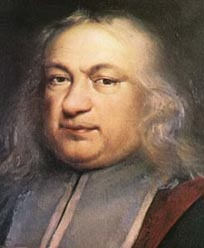
\includegraphics[scale=0.5]{image_chapitres/fermat.jpg}

\unnumberedcaption{Pierre de \textsc{fermat}} 
\end{wrapfigure}

Les statistiques mathématiques s'appuyaient sur les premiers travaux concernant les probabilités développés par \textsc{\textbf{Fermat}} et \textsc{Pascal}. C'est probablement chez Thomas \textsc{Bayes} que l'on vit apparaître un embryon de statistique inférentielle. \textsc{Condorcet} et \textsc{Laplace} parlaient encore de probabilité là où l'on parlerait aujourd'hui de fréquence. Mais c'est à Adolphe \textsc{Quetelet} que l'on doit l'idée que la statistique est une science s'appuyant sur les probabilités.

Pierre-Simon de \textsc{Laplace} fait entrer l'analyse dans la théorie des probabilités dans sa théorie analytique des probabilités de 1812 qui restera longtemps un monument. Son livre donne une première version du théorème central limite qui ne s'applique alors que pour une variable à deux états, par exemple pile ou face mais pas un dé à 6 faces. Il faudra attendre 1901 pour en voir apparaître la première version générale par \textsc{Liapounov}. C'est aussi dans ce traité qu'apparaît la méthode de Laplace pour l'évaluation asymptotique de certaines intégrales.

Sous l'impulsion de textsc{Quetelet}, qui ouvre en 1841 le premier bureau statistique le Conseil Supérieur de Statistique, les statistiques se développent et deviennent un domaine à part entière des mathématiques qui s'appuie sur les probabilités mais n'en font plus partie.

La théorie moderne des probabilités ne prend réellement son essor qu'avec la notion de mesure et d'ensembles mesurables qu'Émile \textsc{Borel} introduit en 1897.
Informatique
 
\PESP{https://fr.wikipedia.org/wiki/Histoire_des_statistiques}
 
\end{His}